\chapter{}
Pouco tempo se passou até que a primeira parcela do financiamento para o plantio de café no Mato Grosso fosse liberada.
Paulo pediu demissão do emprego e fomos à luta.
Um punhado de gente se lançara conosco na aventura.
Poucos, porém, encararam a Bodoquena, ainda que, a rigor, fosse a única região compatível com as especificações exigidas pelo IBC\footnote{Então, Instituto Brasileiro do Café. Hoje, o Conselho Deliberativo de Política do Café, do Ministério da Agricultura, ocupa seu lugar.}.
Muitos produtores preferiram ficar ali mesmo nas imediações de Campo Grande e não se sabe como conseguiram convencer os fiscais do órgão de que aqueles campos vermelhos, baixos e escassos de água, quentíssimos no verão, atendiam perfeitamente às necessidades de altitude e temperatura da cultura exigente.
Alguns, nos olhavam com ceticismo.
O solo da serra era fantástico, era sabido, mas esse mesmo solo no período das chuvas transformava-se num atoleiro intransponível.
E havia o risco de geada.
E a distância.
Se uma peça de trator quebrasse, entre o ir e voltar de Campo Grande para o necessário reparo era um mês de serviço parado.
A verdade, haveríamos de descobrir depois, é que boa parte dessa gente não estava minimamente interessada em produzir café.
O que queriam era apenas o dinheiro fácil e abundante.
O próprio pai do Léo, o lendário Leôncio Brito, dono de extensas pastagens e de muito gado no Campo dos Índios e na Bodoquena, aconselhou:
\textit{``-- Agora que teve a sorte de botar a mão nesse monte de dinheiro, compre tudo em gado, solte no meio da plantação e quando os fiscais do I.B.C.
aparecerem, diga-lhes que a cerca caiu e os bois pastaram todo o cafezal''}.

Ficamos cerca de um mês e meio hospedados com Léo e Lisete na Fazenda Brejão.
Lá tomei contato com mais alguns costumes do lugar.
Lisete vinha de uma família culta de Piracicaba, que ainda realizava saraus musicais em torno de um piano e descendia de Tobias Barreto de Menezes, o primeiro filósofo brasileiro.
Sua adaptação vinha sendo sofrida.
Naquelas paragens, mulher se mantinha na retaguarda.
Não sentava com o marido à mesa, pois era de preceito que ele comesse no galpão, com seus peões.
Ela apenas comandava o serviço na cozinha e servia à mesa com as criadas.
Quando os sogros não estavam pela fazenda, por insistência de Lisete, Léo ainda afrontava o costume, almoçando na companhia dela.
Mas, quando o velho Leôncio e a mulher chegavam a tradição se impunha e a minha pobre amiga tinha que se conformar em ficar no borralho, na companhia da sogra.


O dia se iniciava ainda na madrugada com o ``quebra-torto'', uma refeição que incluía carne de charque frita ou assada, acompanhada de mandioca cozida, após o que se seguia uma rodada de ``tereré'', um mate preparado com água gelada e bebido na cuia comum que passava de mão em mão, para selar a camaradagem que devia reinar entre todos, fossem patrões ou empregados.
O leite era apreciado também, principalmente sob a forma de coalhada, adoçada às vezes.
Em vez de pão, era mais comum encontrar um biscoito feito de polvilho, duríssimo, chamado ``chipa'' e parecido com outro, também duro de roer, este feito de farinha de milho e estranhamente batizado de ``sopa paraguaia''.
Por volta das dez, o almoço era servido e o cardápio se mantinha mais ou menos igual, com o acréscimo de uns raros legumes ou verduras.
E tudo cozido na ``graxa'', isto é, sebo de boi, o que obrigava a enfiar a comida escaldando na boca, pois se ela esfriasse apenas levemente, só despegava do céu da boca e dos dentes à força de suco de limão, conforme me ensinaram.
Ao jantar, às quatro ou cinco horas da tarde, de novo retornavam variações de charque acompanhadas da indefectível mandioca e o dia terminava na roda de tereré.
Em que pese a pouca variedade, esses hábitos alimentares somados à vida no campo, com certeza explicavam o vigor daquela gente, sua cor magnífica, o físico privilegiado -- não se via obesos nem raquíticos -- e, principalmente, o fato de não se encontrar desdentados entre eles, o que, naquele tempo, em se tratando de população rural, era espantoso.

Algumas poucas vezes eu ficava no Brejão, fazendo companhia a Lisete.
Na maior parte do tempo, porém, eu preferia ir com Paulo até a nossa fazenda, que, a partir de então, haveria de se chamar Santa Teresa.
Tudo naquela vida era novidade para mim, mas a maior de todas era ver meu marido comandar a transformação daquele pedaço quase virgem de terra num empreendimento de tamanho porte.
Sim, porque havíamos financiado o plantio de nada menos que duzentos e cinquenta mil pés de café!

\begin{figure}
\centering
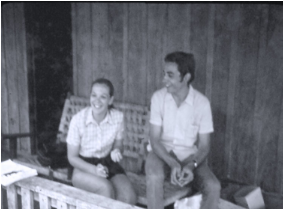
\includegraphics[width=0.8\linewidth]{21/na-santa-teresa.png}
\caption{Na Santa Teresa, na varanda da casa do Benício.}
\end{figure}

Quando Benício deixou a casa da sede, o que levou algum tempo, vimos que ela precisava de alguma reforma.
Alvenaria quase não era usada naquela região pela dificuldade de material, transporte e mão de obra.
As casas eram feitas da madeira abundante que havia por ali.
Duravam bastante, mas precisavam de reparos periódicos.
E naquele momento Paulo tinha mais em que pensar: os trabalhos teriam início com a derrubada da mata, o que significava ir atrás de ``gatos'' confiáveis e se preparar para receber cerca de cem homens de todo tipo e procedência, capazes de encarar a tarefa de pôr abaixo, no machado, árvores enormes, centenárias, como aquelas que tínhamos no alto do paredão e nos fundos da fazenda.
Usava-se também a motosserra, mas com mais parcimônia, porque nem todos sabiam manejá-la e era fácil de quebrar.

Mudamo-nos para uma casinha que Paulo fez anexa ao recém-construído barracão para abrigar equipamentos e ferramentas.
Era também de madeira, porém tinha o luxo de uma serpentina instalada no fogão de lenha que proporcionava banho quente.

\begin{figure}
\centering
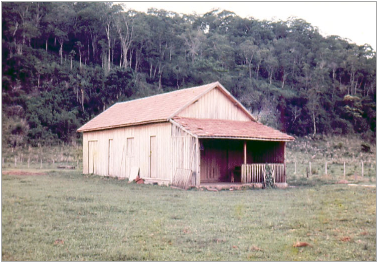
\includegraphics[width=0.8\linewidth]{21/instalações.png}
\caption{Nossas instalações na Santa Teresa.}
\end{figure}

Havia algum tempo, minha cabeça se ocupava continuamente de um problema que nada tinha a ver com toda aquela trabalheira da implantação da fazenda.
Era o seguinte: já ia para ano e meio que estávamos casados e eu não engravidava.
Ora, o meu desejo de ter filhos tinha sido decisivo para revogar minha disposição contrária ao casamento.
Eu sempre quis muito ser mãe.
Nada tenho contra quem resiste à ideia, mas, no meu caso, seria difícil dar um sentido à vida se isso me fosse negado.
Um dia, entretanto, quando eu ainda estava hospedada no Brejão, acordei indisposta.
A visão do café da manhã provocou-me náusea.
A tentativa de almoçar, mais tarde, resultou em vômito incontrolável.
Três dias depois, tudo que eu conseguia engolir eram gomos de lima da Pérsia e água.
Paulo levou-me de volta a Campo Grande, para consultar um médico.
Pensávamos numa infecção intestinal séria.
O médico sorriu.
Não era.
Era gravidez, como o exame confirmou em seguida.
Assim que tive o resultado nas mãos, ali escrito e arrematado pela figurinha da cegonha trazendo no bico um bebê, o enjoo desapareceu instantaneamente para nunca mais voltar.
Em nenhuma das outras quatro gravidezes que se seguiriam àquela.
